\interlude[0]{About cryptology}
\section{About cryptology}

\begin{frame}{To build real-world cryptography solutions}
  \centering
  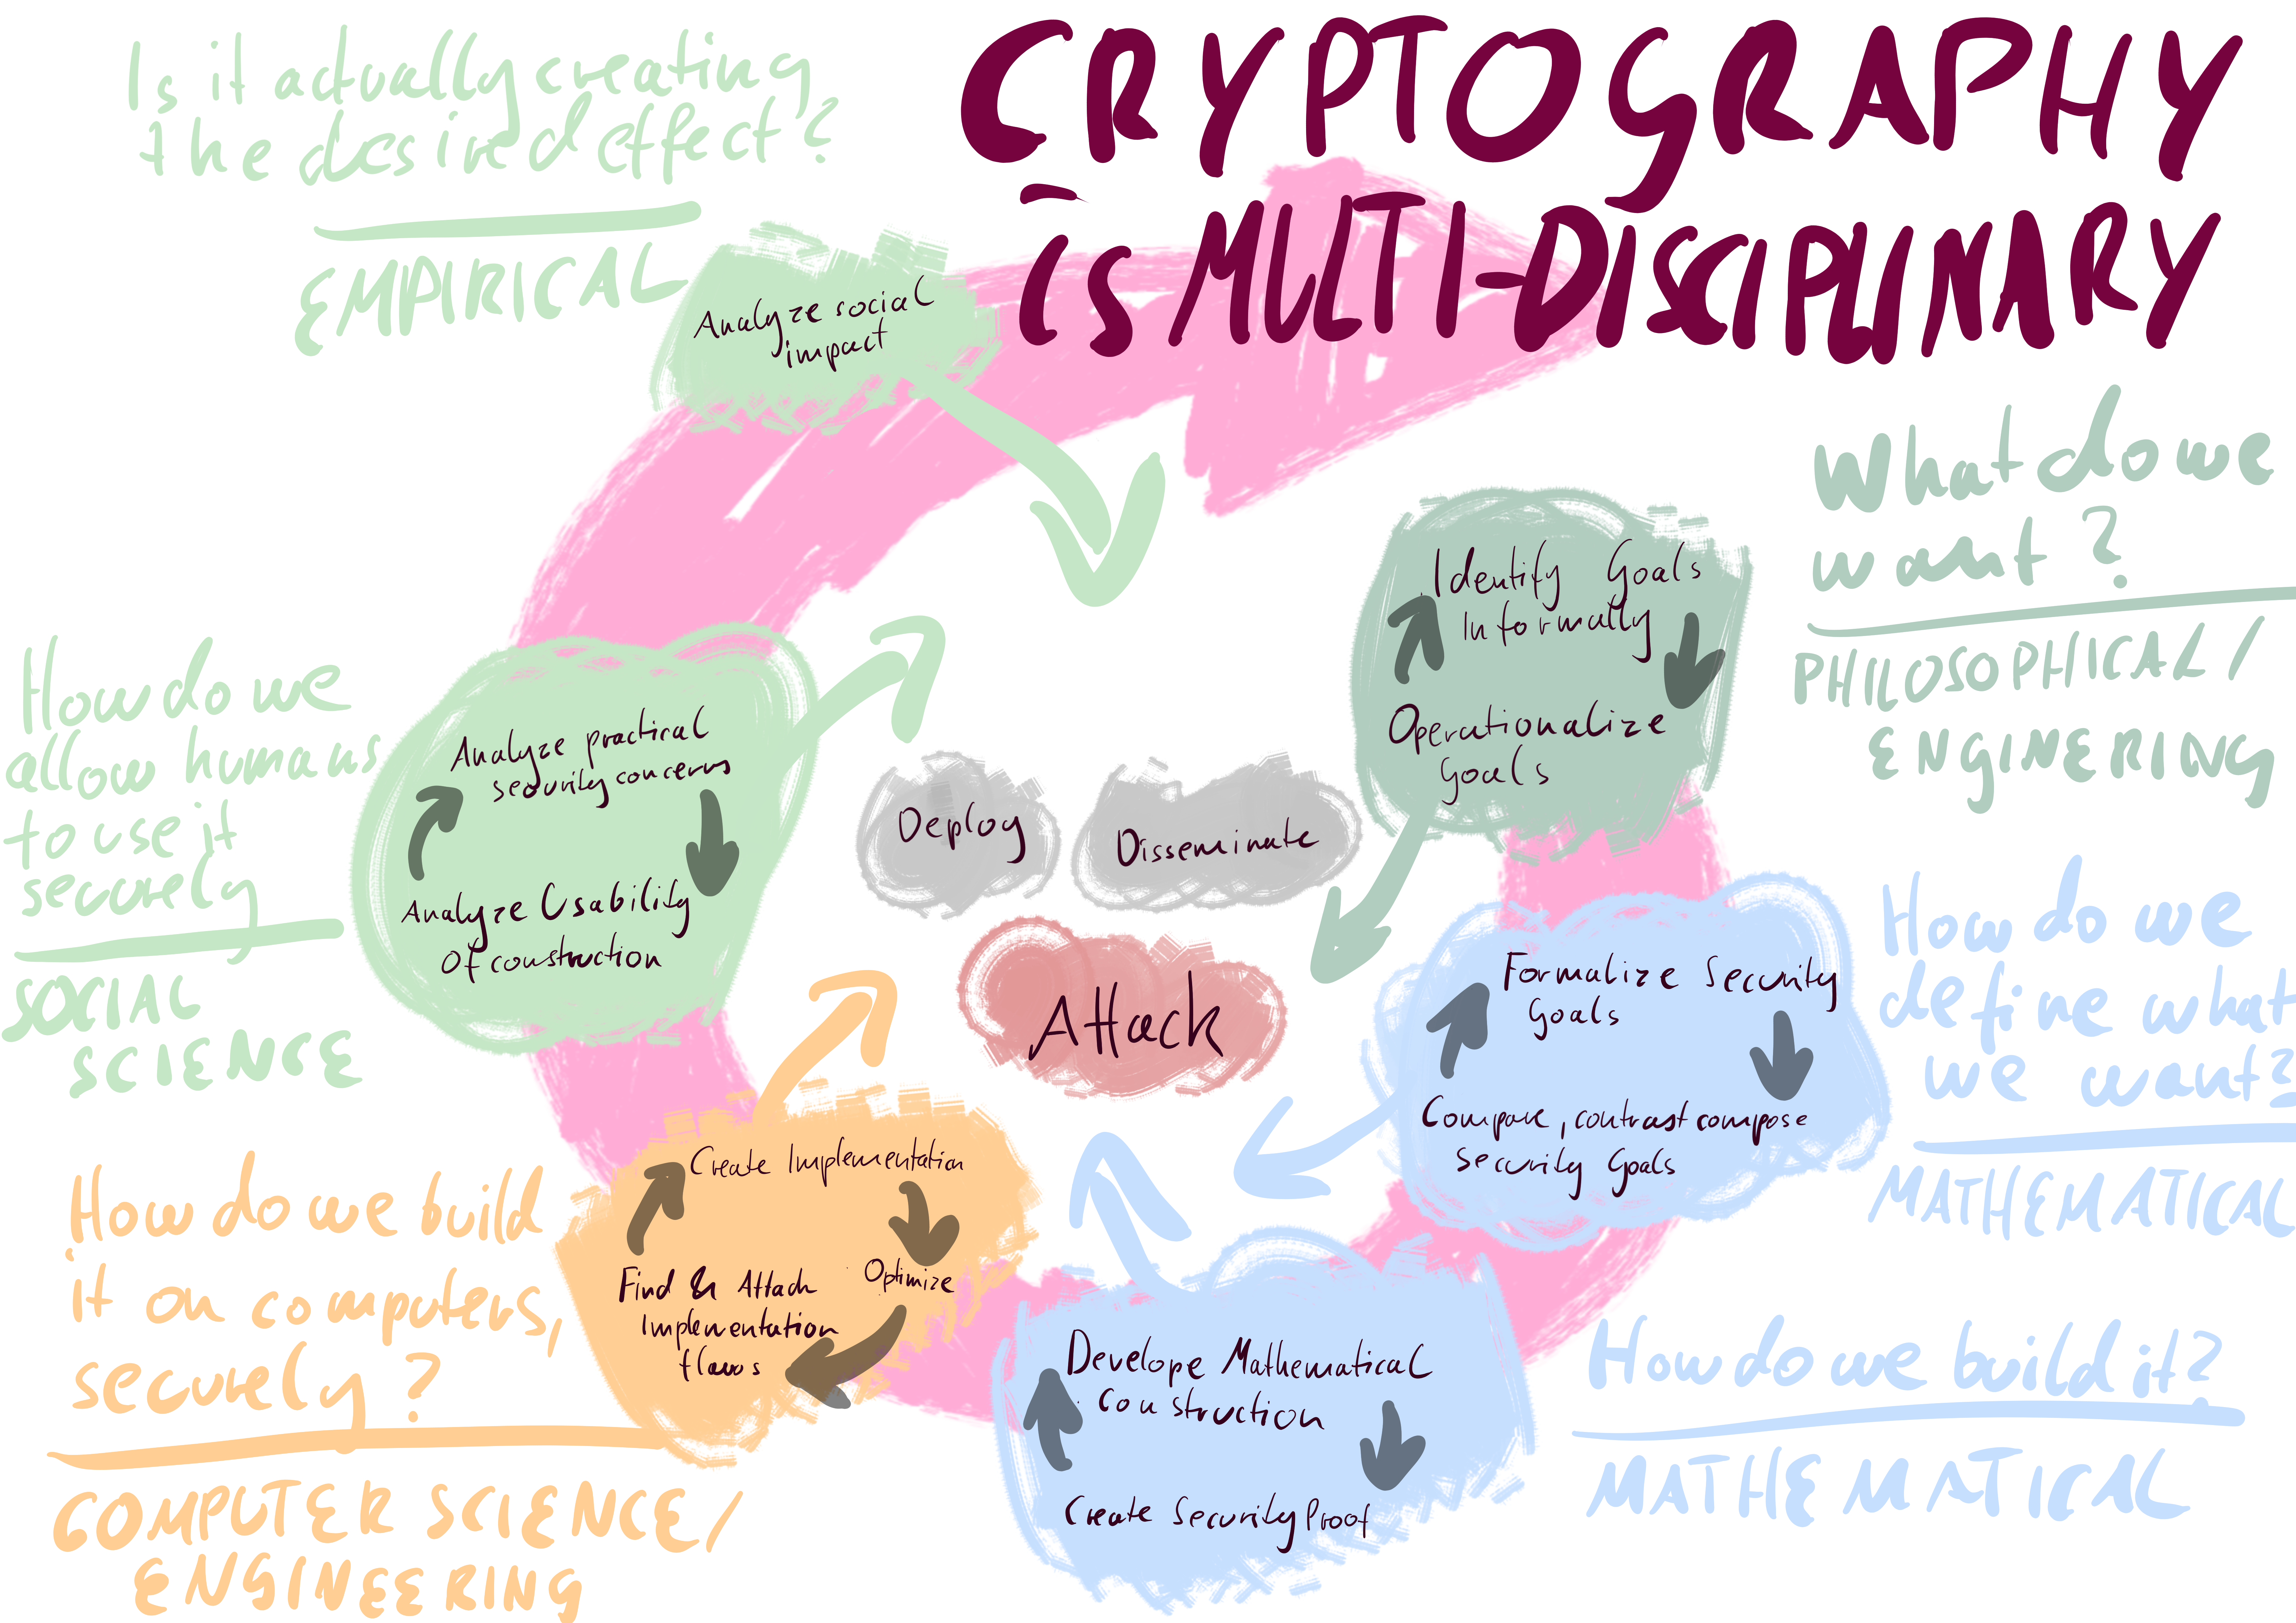
\includegraphics[height=.82\textheight]{graphics/cryptography-is-multidisciplinary-draft.png}
\end{frame}

\begin{frame}{Proofs of security are fundamental: Reduction proofs}
  \small
  Proof by reduction to a well-known mathematical problem \emph{assumed to be hard} or existing cryptographic construction \emph{assumed to be secure}.
  \vfill
  \textbf{If} an attack against my cryptosystem exists,
  \\ \textbf{then} this other cryptosystem can be attacked or this math problem can be solved.
  \vfill
  Proof ad-absurdum:
  \begin{itemize}
    \item Assume an attacker against the new cryptosystem exists
    \item Construct a solution to the underlying math problem using the assumed attacker
  \end{itemize}
\end{frame}

\begin{frame}{Proofs are fundamental: Using information theory}
  \small

  Showing that each \emph{plain text} is plausible for each \emph{ciphertext}.

  \vfill

  Cryptosystem should be formulated as a function:

  $$F : K \times D \to C$$

  \begin{description}
    \item[$K$] Key material; secret information held by the trusted parties
    \item[$D$] Protected information
    \item[$C$] Leaked information; any information known to the attacker after protocol execution
  \end{description}

  Now it needs to be shown, that for every value of the leaked information,
  every value of the protected information is equally plausible.


  $$\forall c : C, d_1 : D, d_2 : D; |\{ k \in K | F(k, d_1) = c \}| = |\{ k \in K | F(k, d_2) = c \}|$$
\end{frame}

\begin{frame}{Practical security is essential}
  \small

  It is not enough to build a system that is secure in theory but vulnerable on real hardware.
  Some dangers include:

  \begin{itemize}
    \item Timing side-channels
    \item Power side-channels
    \item Hardware bugs in the CPU (Rowhammer, Spectre, or Meltdown)
    \item Lack of usability (Implementations that are easy to misuse)
  \end{itemize}
\end{frame}

\setbeamertemplate{background canvas}{\includegraphics[width=\paperwidth]{graphics-repo/comic/kryptoparty-wide}}
\begin{frame}{Implementations and specifications must be open}
  % TODO(karolin): Copy/paste kerkoffs principle
\end{frame}

\setbeamertemplate{background canvas}{}

\begin{frame}{Open-Source \& Open-Science are mandatory}
  \begin{columns}[onlytextwidth,c]
      \begin{column}<only@+|handout:+>{\defaultframetextheight}
        \includegraphics[width=.5\linewidth]{graphics-repo/comic/rosenpass-comic_01-obscurity1.jpg}%
        \includegraphics[width=.5\linewidth]{graphics-repo/comic/rosenpass-comic_01-obscurity2.jpg}

        \includegraphics[width=.5\linewidth]{graphics-repo/comic/rosenpass-comic_01-obscurity3.jpg}%
        \includegraphics[width=.5\linewidth]{graphics-repo/comic/rosenpass-comic_01-obscurity4.jpg}
      \end{column}
		
      \begin{column}<only@.|handout:.>{.4\linewidth}
        Keeping details about a security system secret creates mistrust and risks obscuring obvious security flaws
      \end{column}

      % 2nd overlay
      \begin{column}<only@+|handout:+>{.4\linewidth}
        Cryptography is about creating trust; so peer review and open processes are a crucial part of the process.
      \end{column}
	\hfill
      \begin{column}<only@.|handout:.>{\defaultframetextheight}
        \includegraphics[width=.5\linewidth]{graphics-repo/comic/rosenpass-comic_02-disclosure1.jpg}%
        \includegraphics[width=.5\linewidth]{graphics-repo/comic/rosenpass-comic_02-disclosure2.jpg}
      \end{column}
  \end{columns}
\end{frame}

\begin{frame}{To integrate QKD in cryptology}
  \small
  \begin{itemize}
    \item Integrate with community of cryptography researchers
    \item Use open-source/open-science approach
    \item Define security properties in cryptographic terms to be comparable
    \item \textbf{Use QKD within cryptographic systems}
  \end{itemize}
\end{frame}
